Nesta seção serão apresentados os fundamentos teóricos que dão suporte à realização deste trabalho. As redes neurais artificias, seus principais conceitos, arquiteturas, métodos de aprendizagem e algumas aplicações são discorridas na Seção \ref{subsec:rna}. Os conceitos elementares sobre as técnicas de \textit{Machine Learning} conhecidas como \textit{Deep Learning} encontram-se na Seção \ref{subsec:deep}. Na Seção \ref{subsec:cnn} são descritas as características das redes neurais utilizadas pela técnica de \textit{Deep Learning}, as Redes Neurais Convolucionais. Por fim, as tecnologias utilizadas para a realização deste trabalho são apresentadas na Seção \ref{subsec:tecnologias}.

\subsection{Redes Neurais Artificiais} \label{subsec:rna}
% Ideia geral

As \emph{Redes Neurais Artificiais} (RNAs) são modelos computacionais inspirados na capacidade de processamento de informações do cérebro humano \cite{ref:rojas}. De acordo com esta ideia, as RNAs possuem unidades de processamento simples, denominadas \emph{neurônios artificiais}, dispostos em camadas interconectadas por ligações associadas a coeficientes numéricos, chamados \emph{pesos} \cite{ref:faceli}. As RNAs são capazes de aprenderem padrões complexos a partir dos dados e prever resultados para exemplos não conhecidos, o que demonstra a sua capacidade de generalização \cite{ref:haykin}.

% Neurônio Artificial

O neurônio artificial é a unidade fundamental na construção de RNAs, tendo sido inspirado no seu análogo biológico. Segundo Rosenblatt, existe um conjunto de $m$ entradas, equivalentes aos dendritos de um neurônio biológico, por onde os sinais são introduzidos \cite{ref:rosenblatt}. Associa-se um peso a cada entrada, representando a relevância referente a uma conexão sináptica. Há também o peso $w_0$, um termo de polarização criado com a intenção de estabelecer um limiar de ativação para cada neurônio. Este peso corresponde à entrada \emph{bias}, cujo valor é sempre unitário. Pode-se então definir um vetor de entradas $X = [+1, x_1, x_2, \ldots, x_m]$ e um vetor de pesos $W = [w_0, w_1, \ldots, w_m$]. As entradas e pesos são combinados por meio de uma função $\phi: \mathbbm{R}^{m+1} \rightarrow \mathbbm{R}$, que é geralmente a soma ponderada das entradas e pesos, conforme Equação \ref{eq:somaPonderada}. Este modelo de neurônio encontra-se ilustrado na Figura \ref{img:neuronioArtificial} \cite{ref:patrick-tcc}.

\begin{equation}
\phi(X,W) = \sum_{i =0}^m x_i \cdot w_i. \label{eq:somaPonderada}
\end{equation}

\begin{figure}[h!]
	\centering
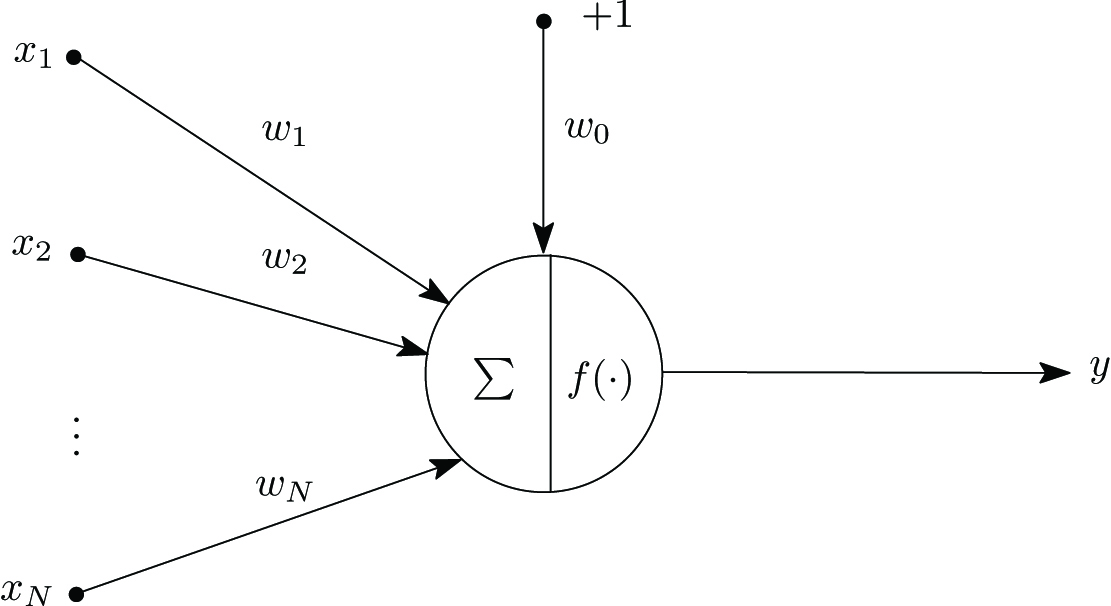
\includegraphics[width=0.6\textwidth]{./img/neuron}
\caption{Neurônio artificial: a combinação linear das entradas \emph{x} ponderadas pelos pesos \emph{w} é transformada pela função de ativação \emph{f} na saída \emph{y}.}
\label{img:neuronioArtificial}
\end{figure}

% Funções de ativação

A função $f$ é chamada de \emph{função de ativação} e fornece a resposta de um neurônio para uma dada entrada. Esta função precisa ser monotônica e contínua, podendo comumente ser as funções identidade, sigmóide, tangente hiperbólica, ou a retificada linear (ReLU) \cite{ref:JAI-2017}. Estas funções encontram-se representadas na Figura \ref{img:funcs_ativacao}.

\begin{figure}[h!]
	\centering
	\subfloat[Função identidade. \label{img:func_id}]{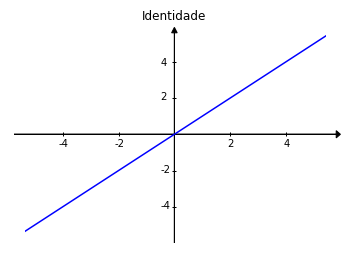
\includegraphics[width=0.4\linewidth]{./img/id}}
	\subfloat[Função sigmóide.\label{img:func_sigmoide}]{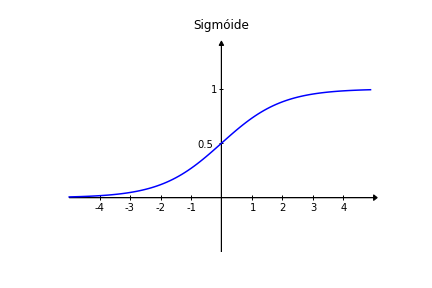
\includegraphics[width=0.4\linewidth]{./img/sigmoide}}\\
	\subfloat[Função tangente hiperbólica. \label{img:func_tanh}]{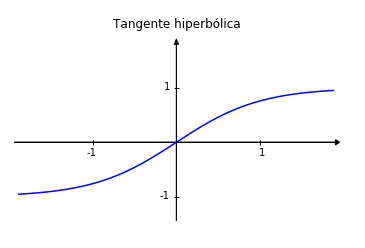
\includegraphics[width=0.4\linewidth]{./img/tanh}}
	\subfloat[Função retificada linear.\label{img:func_relu}]{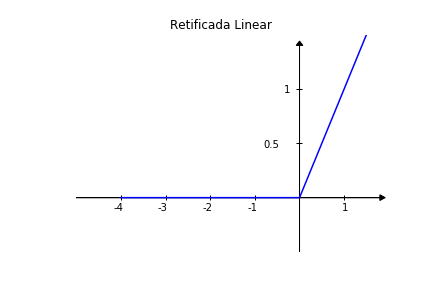
\includegraphics[width=0.4\linewidth]{./img/relu}}
	\label{img:funcs_ativacao}
	\caption{Exemplos de diferentes funções de ativação.}
	\label{img:funcs_ativacao}
\end{figure}

% Camadas ocultas

Neurônios artificiais individuais têm uma capacidade computacional limitada, independentemente da função de ativação escolhida, pois resolvem apenas problemas linearmente separáveis. No entanto, um conjunto de neurônios artificiais conectados na forma de uma rede -- \emph{rede neural artificial} -- adquirem a capacidade de resolver problemas de elevada complexidade \cite{ref:teresa}. A alternativa mais utilizada para resolver estes problemas é distribuir os neurônios em uma ou mais camadas conhecidas como  camadas ocultas \cite{ref:faceli}. Segundo Cybenko, uma rede com uma camada oculta pode implementar qualquer função contínua e uma rede com duas camadas ocultas permite a aproximação de qualquer função \cite{ref:cybenko}.

% Multilayer Perceptron

As RNAs do tipo Perceptron Multicamadas (MLP, do inglês \emph{Multilayer Perceptron}) apresentam uma camada de entrada, uma ou mais camadas ocultas e uma camada de saída. Uma das principais características de uma rede MLP é o seu alto grau de conectividade entre os neurônios, cuja intensidade está associada aos pesos da rede.

Cada neurônio em uma rede MLP atua ponderando as entradas recebidas dos neurônios de uma camada anterior a ele conectados, produzindo como saída um valor, resultante de sua função de ativação, que é propagado às camadas seguintes da rede neural. Conforme exemplificado na Figura \ref{img:rede-mlp}, a combinação das atuações individuais desempenhadas por cada neurônio da rede que define a atuação associada à RNA como um todo \cite{ref:teresa,ref:faceli,ref:haykin}.


\begin{figure}[h!]
	\centering
	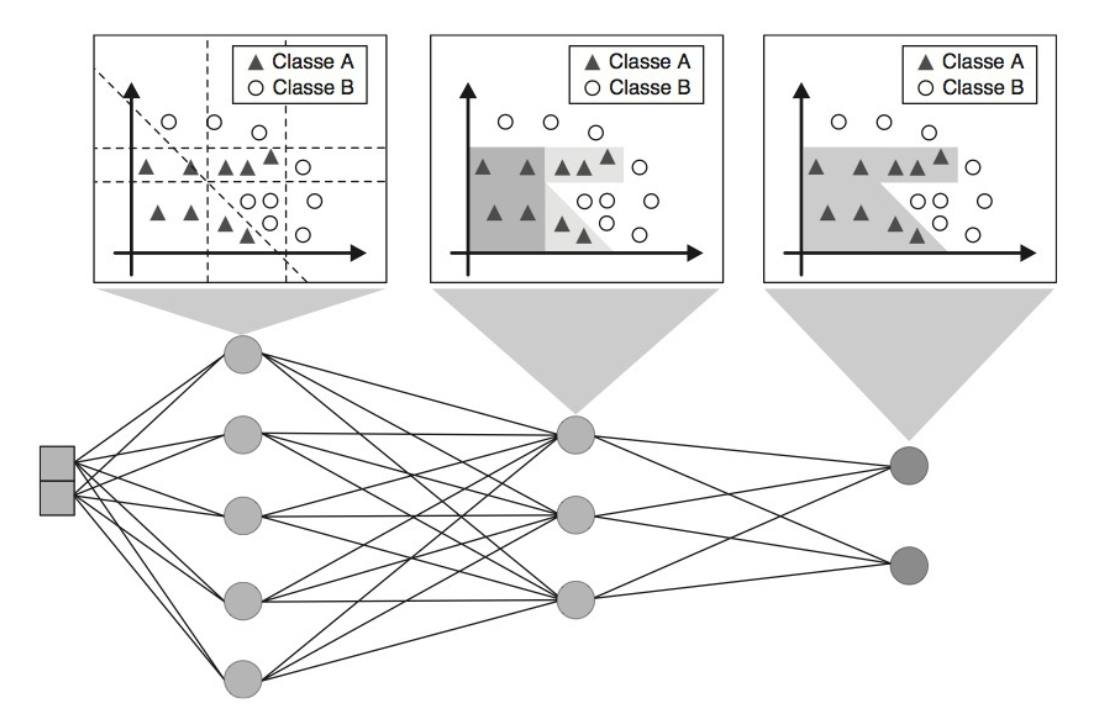
\includegraphics[width=1\textwidth]{./img/rede-mlp}
	\caption{Papel desempenhado pelos neurônios das diferentes camadas de uma rede MLP. Fonte: \cite{ref:faceli}.}
	\label{img:rede-mlp}
\end{figure}

% Aprendizado

Uma importante característica das RNAs é a sua capacidade de aprender por meio de exemplos. O processo de \emph{aprendizado} de uma rede neural consiste em sucessivos ajustes de pesos associados aos seus neurônios, de modo a aprimorar seu desempenho de acordo com um critério pré-estabelecido. Tais ajustes são realizados por algoritmos de treinamento formados por um conjunto de regras bem definidas que especificam quando e como deve ser alterado o valor de cada peso. Diversos algoritmos de aprendizado foram propostos, dentre os quais se destacam aqueles que seguem o paradigma de \emph{aprendizado supervisionado} \cite{ref:faceli,ref:patrick-tcc}.

% Paradigmas de aprendizado

O aprendizado supervisionado ajusta os pesos aplicando um conjunto de exemplos de treinamento rotulados. Cada exemplo consiste em um sinal de entrada associado à sua resposta alvo desejada. A cada padrão de entrada submetido à rede, compara-se a resposta desejada com a resposta calculada, ajustando-se os pesos das conexões para minimizar o erro \cite{ref:haykin}.

% Backpropagation

O algoritmo mais utilizado para o treinamento de redes MLP é o algoritmo \emph{backpropagation}, também chamado de retropropagação do erro ou ainda regra delta generalizada. Este algoritmo respeita o aprendizado supervisionado em que os pesos são modificados e ajustados para reduzir a distância entre a resposta desejada e a resposta produzida pela rede \cite{ref:haykin}. O treinamento é constituído da iteração de duas fases, uma fase para frente (\emph{forward}) e uma fase para trás (\emph{backwards}) \cite{ref:faceli}. A fase \emph{forward}, que compreende o fluxo da informação a partir da entrada até a saída da rede, é utilizada para produzir uma saída para um dado sinal de entrada. A fase \emph{backwards}, com fluxo da informação da saída da rede em direção à entrada, utiliza a diferença entre as saídas desejada e produzida para atualizar os pesos das conexões entre os neurônios e assim minimizar o erro \cite{ref:teresa}. Os ciclos de apresentação dos dados de treinamento e eventuais ajustes de pesos no \emph{backpropagation} são iterados até que seja atingido um critério de parada como, por exemplo, um número máximo de ciclos ou uma taxa máxima de erro \cite{ref:faceli}.


% Aplicações

As RNAs são modelos computacionais com ampla aplicação na resolução de problemas de previsão. Algumas aplicações utilizam RNAs para predição de condições climáticas, como em \cite{ref:apl-clima1} e \cite{ref:apl-clima2}, em que se deseja prever precipitações de chuva de determinados locais. Diversas outras aplicações de RNAs dizem respeito à classificação de padrões. Dentre as aplicações na área de classificação financeira, uma das mais bem sucedidas é a análise de crédito \cite{ref:teresa}. Além disso, as RNAs também são muito utilizadas para diagnósticos médicos, como em \cite{ref:apl-diagnostico1} e \cite{ref:apl-diagnostico2}. Outras aplicações tratam de reconhecimento de caracteres \cite{ref:apl-caracteres}, robótica \cite{ref:apl-robotica}, jogos \cite{ref:apl-jogos}, comunicação \cite{ref:meu-artigo}, dentre outros.

\subsection{\textit{Deep Learning}} \label{subsec:deep}
\emph{Deep Learning} (DL), ou Aprendizado Profundo, é uma subárea do AM especialmente baseada na utilização de RNAs com uma grande quantidade de camadas e neurônios para aprender padrões complexos em um vasto volume de dados \cite{ref:chollet,ref:khan,ref:gulli}. Por meio do reconhecimento de padrões, os modelos baseados em DL são capazes de reconhecer, traduzir, sintetizar e até prever padrões das mais diferentes naturezas \cite{ref:JAI-2017}.

As técnicas de DL têm sido aplicadas com êxito em muitos problemas, especialmente considerando dados de alta dimensionalidade, a exemplo de imagens e vídeos, e contextos em que há uma grande disponibilidade de exemplos  \cite{ref:JAI-2017,ref:khan}. Os modelos de DL têm se destacado, por exemplo, em muitas aplicações de saúde, especialmente considerando a detecção automática de padrões em imagens médicas para fins diagnósticos \cite{ref:yang}. O desafio
\emph{ImageNet Large Scale Visual Recognition Challenge}, de caráter anual realizado desde 2010, também têm promovido a proposição e competição de modelos de vanguada para fins de detecção de objetos e classificação de imagens em larga escala, contribuindo para o desenvolvimento do estado da arte em VC \cite{ref:image-net}.

Os modelos e técnicas de DL têm sido aplicados em tarefas de aprendizado supervisionado e não supervisionado, em que as redes neurais convolucionais têm sido o modelo mais proeminente. A seção a seguir apresenta o detalhamento deste modelo, suas características e conceitos associados.

\subsubsection{Redes Neurais Convolucionais} \label{subsec:cnn}
As \textit{Redes Neurais Convolucionais}, do inglês \textit{Convolutional Neural Networks} (CNNs), são modelos de redes neurais especializados em processamento de dados compostos pela união de vários segmentos elementares denominados camadas \cite{ref:goodfellow}. Cada camada possui uma finalidade específica e implementa uma determinada funcionalidade básica como convolução, normalização, \textit{pooling}, etc \cite{ref:khan}.

A camada convolucional é a camada mais importante de uma CNN e utiliza uma operação matemática linear chamada \textit{convolução} \cite{ref:goodfellow}. O processo de convolução é aplicado em um conjunto de \textit{filtros} e uma dada entrada para gerar uma saída conhecida como \textit{mapa de características}. Cada filtro consiste em uma matriz de números discretos que representam os pesos da CNN \cite{ref:khan}.

%cálculo da convolução


A camada convolucional recebe um volume de entrada de largura $w_{in}$, altura $h_{in}$ e profundidade $d_{in}$ e pode possuir um preenchimento  $p$ de zeros (\textit{zero-padding}), aplicado ao redor da entrada. Essa entrada é processada por $k$ filtros que representam os pesos e as conexões da CNN. Cada filtro possui uma extensão espacial $e$, que é igual ao valor da altura e da largura do filtro, e um \textit{stride} $s$, que é a distância entre as aplicações consecutivas do filtro no volume de entrada. A saída da camada de convolução é um volume de largura $w_{out}$ calculado conforme a Equação \ref{eq:wout}, altura $h_{out}$ conforme Equação \ref{eq:hout}  e profundidade $d_{out}$ igual a $k$ \cite{ref:buduma}. 

\begin{equation}
w_{out} = \frac{w_{in} - e + 2p}{s} +1 \label{eq:wout}
\end{equation}

\begin{equation}
h_{out} = \frac{h_{in} - e + 2p}{s} +1 \label{eq:hout}
\end{equation}

\subsubsection{Arquiteturas Canônicas de Redes Neurais Convolucionais} \label{subsubsec:arquiteturas}
Como mencionado anteriormente, o desafio anual \emph{ImageNet Large Scale Visual Recognition Challenge} (ILSVRC) têm tido um papel protagonista no desenvolvimento de soluções em DL, pois têm promovido um contexto para proposição e comparação de algumas das arquiteturas de CNNs mais bem sucedidas para problemas de detecção de objetos e classificação de imagens em larga escala \todo{Incluir citação}.

\todo{Uma figura da evolução da competição ano a ano? Quais as métricas? Qual o ganho? Mencionar um pouco mais a contribuição desta competição}

\todo{Como diz no site do ILSVRC: Citation
When reporting results of the challenges or using the datasets, please cite:
Olga Russakovsky*, Jia Deng*, Hao Su, Jonathan Krause, Sanjeev Satheesh, Sean Ma, Zhiheng Huang, Andrej Karpathy, Aditya Khosla, Michael Bernstein, Alexander C. Berg and Li Fei-Fei. (* = equal contribution) ImageNet Large Scale Visual Recognition Challenge. IJCV, 2015. paper | bibtex | paper content on arxiv | attribute annotations. Lá tem o bibtex. Trocar as referências ao longo do texto}

Embora os conceitos das camadas de uma CNN estejam bem estabelecidos e sejam de conhecimento geral, nem sempre é uma tarefa fácil propor uma rede neural deste tipo para um determinado cenário. Assim, uma consequência positiva da realização do ILSVRC é promover a difusão das arquiteturas de destaque na competição, as quais passam ser conhecidas e adaptadas pela comunidade acadêmica e tecnológica na resolução de diversos outros problemas. Considerando esta importância e potencial de aproveitamento de soluções, a seguir são apresentadas algumas destas arquiteturas canônicas.


\paragraph{LeNet} Yann le Cun desenvolveu, em 1990, uma das primeiras arquiteturas utilizadas para o reconhecimento de dígitos manuscritos, a LeNet. Vencedora do ILSVRC 2010, esta arquitetura é composta por três camadas convolucionais alternadas com camadas de \textit{pooling} seguidas de duas FCLs conforme representado na Figura \ref{img:lenet} \cite{ref:sewak,ref:khan}.

\begin{figure}[!ht]
	\centering
	\caption{Arquitetura LeNet de CNN. Fonte: \cite{ref:khan}.}
	\label{img:lenet}
	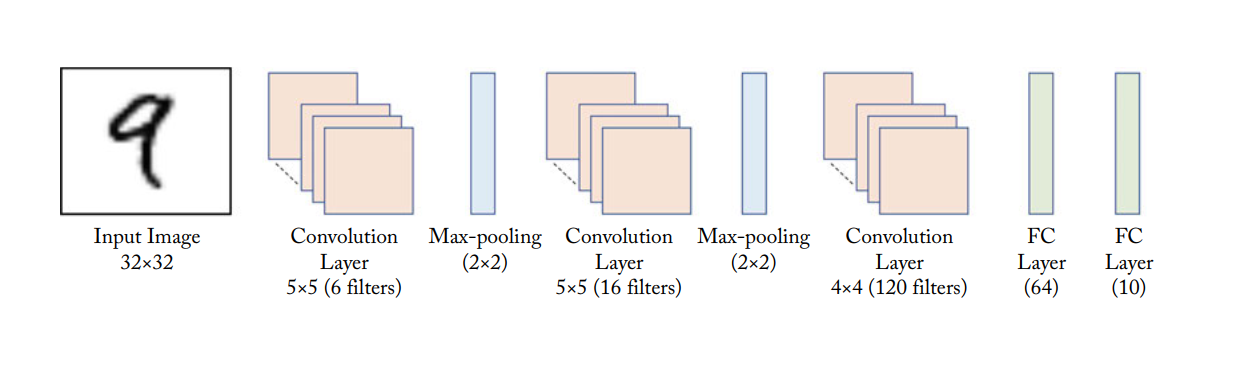
\includegraphics[width=1\textwidth]{./img/lenet}
\end{figure}


\paragraph{AlexNet} Em 2012, a vencedora do ILSVRC foi a arquitetura proposta por Alex Krizhevsky, conhecida como AlexNet, ilustrada na Figura \ref{img:alexnet}. A AlexNet é mais profunda e uma versão muito mais ampla da arquitetura LeNet \cite{ref:satapathy}. A principal diferença entre a AlexNet e as CNNs predecessoras é a sua maior profundidade, que lida muito bem com sua grande quantidade de parâmetros, além da utilização de artifícios como \textit{dropout} e \textit{data augmentation}. As cinco primeiras camadas da arquitetura AlexNet são camadas de convolução e \textit{pooling} alternadas de forma similar à LeNet, porém, seguem-se mais duas camadas uma convolucional e uma de\textit{pooling}. As três últimas camadas são FCL, mas além destas existem camadas \textit{dropout} que ajudam à reduzir \textit{overfiting} \cite{ref:khan}. \todo{Acho que a citação para alexnet está errada.}

\begin{figure}[!ht]
	\centering
	\caption{Arquitetura da AlexNet. Fonte: \cite{ref:khan}.}
	\label{img:alexnet}
	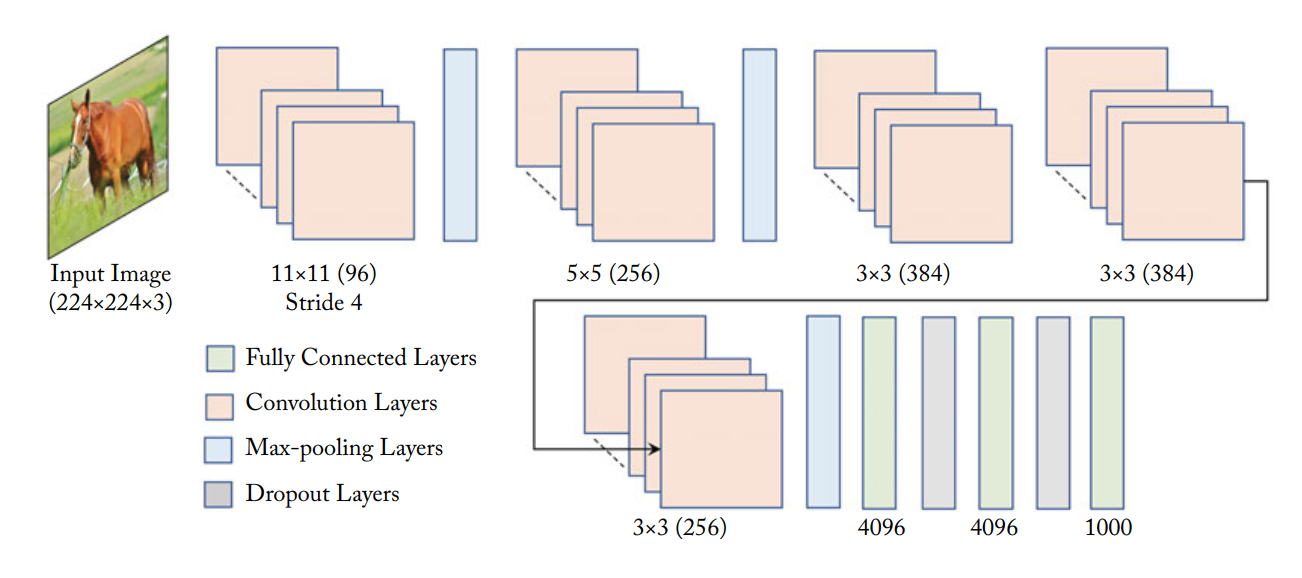
\includegraphics[width=1\textwidth]{./img/alexnet}
\end{figure}

\paragraph{VGGNet} A arquitetura VGGNet é uma das arquiteturas mais populares desde sua criação em 2014, apesar de não ter sido a vencedora do ILSVRC realizado no respectivo ano. A razão de sua popularidade se dá especialmente em virtude do uso de pequenos filtros de convolução, diminuindo o número de parâmetros ajustáveis e, por conseguinte, aumentando a eficiência do treinamento. A arquitetura VGGNet usa estritamente fitros de convolução de dimensão $3 \times 3$ combinados com camadas de \textit{pooling} para extração de características e um conjunto de três FCLs. Além das camadas de convolução, \textit{pooling} e das camadas conectadas, esta arquitetura também possui as camadas \textit{dropout} como pode ser observado na Figura \ref{img:vggnet} \cite{ref:khan}.

\begin{figure}[!ht]
	\centering
	\caption{Arquitetura VGGNet. Fonte: \cite{ref:khan}.}
	\label{img:vggnet}
	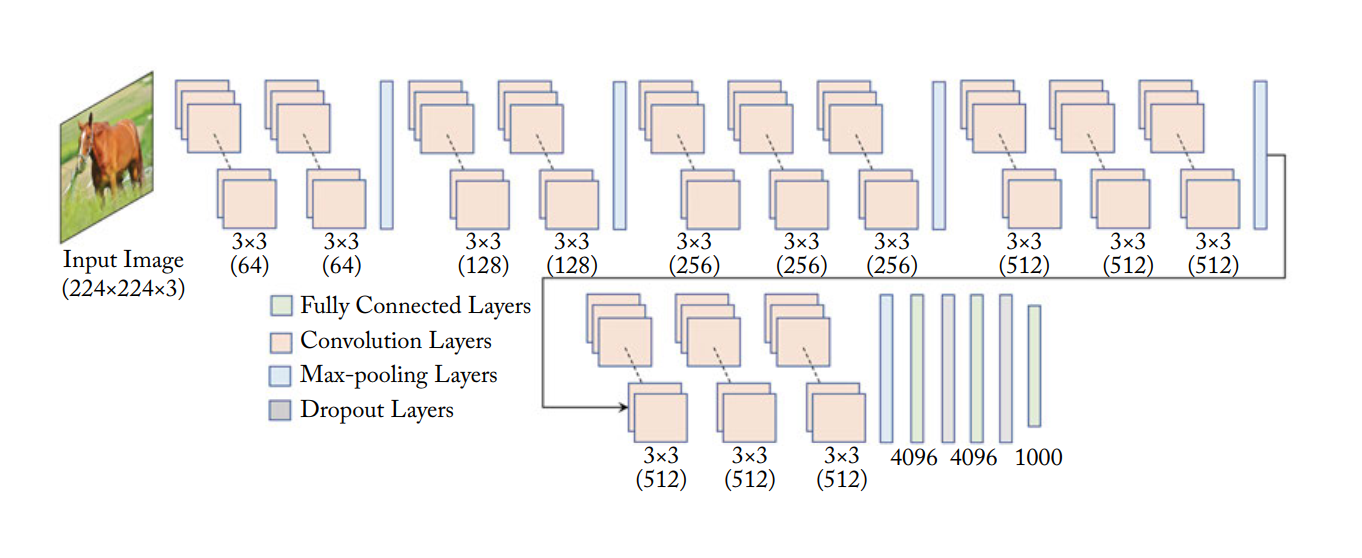
\includegraphics[width=1\textwidth]{./img/vggnet}

\end{figure}

\paragraph{GoogLeNet} Desenvolvida pela empresa Google e vencedora do ILSVRC 2014, a arquitetura GoogLeNet possui $22$ camadas baseadas em um módulo elementar chamado \emph{Inception Module}. O processamento desses módulos ocorre de forma paralela, diferentemente do processamento sequencial das arquiteturas discutidas anteriormente. A ideia central da arquitetura GoogLeNet é paralelizar os módulos e combinar as características da saída sem se preocupar com as funções individuais de cada camada. No entanto, essa abordagem resulta em um mapa de características com muitos elementos, mas para contornar este problema, após a execução do primeiro módulo, a rede realiza uma redução de dimensionalidade utilizando uma FCL antes de continuar o processo de treinamento \cite{ref:khan}. A representação da arquitetura GoogLeNet encontra-se na Figura \ref{img:googlenet}.

\begin{figure}[!ht]
	\centering
	\caption{Arquitetura GoogLeNet. Fonte: \cite{ref:khan}.}
	\label{img:googlenet}
	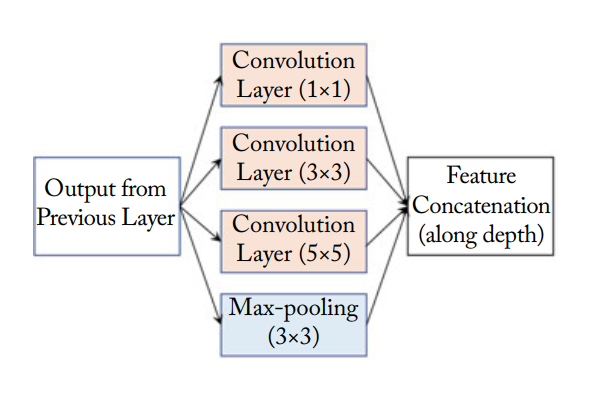
\includegraphics[width=0.6\textwidth]{./img/googlenet}

\end{figure}


\subsection{\textit{Transfer Learning}} \label{subsec:transfer}
\emph{Transfer Learning} (TL), ou Transferência de Conhecimento, é uma poderosa técnica de DL a qual possui diversas aplicações em diferentes domínios \cite{ref:gulli}. Ao invés de estruturar uma arquitetura de uma CNN e treiná-la por completo, esta técnica permite reutilizar uma rede pré-treinada e adaptá-la a um novo conjunto de dados \cite{ref:sewak}. Modelos que foram pré-treinados utilizando um vasto e genérico conjunto de dados conseguem capturar características universais, como por exemplo curvas e arestas, em suas primeiras camadas \cite{ref:zaccone}.

As técnicas de TL podem ser utilizadas de diferentes maneiras, baseando-se nas arquiteturas das CNNs. Existem alguns modelos disponíveis para aplicações que foram pré-treinados utilizando as principais arquiteturas canônicas de CNN e aprenderam as características de grandes conjuntos de dados bastante conhecidos, como o ImageNet e o Places205 \cite{ref:image-net,ref:places205}. Para diferentes tarefas, esses modelos podem ser alterados modificando a camada de saída e fazendo um retreinamento nas últimas camadas das redes para se obter o aprendizado desejado \cite{ref:khan}. 


\subsection{Espaço de Cores CIELab}

\subsection{Tecnologias Utilizadas} \label{subsec:tecnologias}
As tecnologias e bibliotecas predominantemente utilizadas neste trabalho envolvem e s�o compat�veis com a linguagem de programa��o Python, pois esta tem se destacado amplamente em projetos de AM em diversos cen�rios. Esta � uma linguagem de programa��o interpretada, interativa, multi-paradigma,  de alto n�vel, multi-plataforma, com uma sintaxe simples e c�digo aberto, idealizada por Guido van Rossum no in�cio da d�cada de 1990 \cite{ref:python}.

Para o processamento das imagens em termos de redimensionamento, persist�ncia, mudan�a e consulta do espa�o de cores, as bibliotecas \texttt{PIL} (Pillow) e \texttt{colormath} tiveram um papel protagonista \cite{lib:pillow,lib:colormath}. No tocante � manipula��o de arquivos, contemplando abertura, leitura e busca por extens�es similares, as bibliotecas \texttt{os} e \texttt{glob} foram utilizadas \cite{lib:os,lib:glob}. A manipula��o do conjunto de imagens e de suas respectivas representa��es matriciais ficou por conta da \texttt{numpy}, uma biblioteca fundamental para computa��o cient�fica que � extremamente poderosa para gerenciamento e altera��es de matrizes de muitas dimens�es \cite{lib:numpy}.  Ademais, no que diz a respeito do treinamento e testes dos modelos de AM, as bibliotecas \texttt{scikit-learn} e \texttt{keras} foram consideradas, em que a primeira teve um papel principal nos c�lculos autom�ticos das m�tricas de desempenho e a segunda nos modelos de DL com par�metros previamente configurados \cite{lib:scikit,lib:keras}.

Por fim, a infra-estrutura de computa��o em nuvem provida pelo Google Cloud Platform (GCP) totalmente voltada para projetos de AM foi essencial para o desenvolvimento deste projeto. As m�quinas virtuais oferecidas pela plataforma aumentaram o poder computacional acess�vel possibilitando um processamento mais favor�vel ao cen�rio em quest�o. A manipula��o e pr�-processamento do conjunto �ntegro de imagens, o treinamento dos modelos de DL e a fase de an�lise desses modelos foram executados em inst�ncias dispon�veis pelo GCP tendo em vista os recursos de mem�ria e processamento necess�rios \cite{tec:gcloud}.

